% LTeX: enabled=false
\documentclass[a4paper,10pt,oneside]{article}

\usepackage{placeins}

\makeatletter
\AtBeginDocument{%
  % Modifying section command to include FloatBarrier
  \expandafter\renewcommand\expandafter\section\expandafter
    {\expandafter\@fb@secFB\section}%
  % Modifying subsection command to include FloatBarrier
  \expandafter\renewcommand\expandafter\subsection\expandafter
    {\expandafter\@fb@secFB\subsection}%
  
  \newcommand\@fb@secFB{\FloatBarrier
    \gdef\@fb@afterHHook{\@fb@topbarrier \gdef\@fb@afterHHook{}}}%
  
  \g@addto@macro\@afterheading{\@fb@afterHHook}%
  \gdef\@fb@afterHHook{}%
}
\makeatother

\usepackage[english]{babel}

\usepackage[T1]{fontenc}

\usepackage[utf8]{inputenc}

\usepackage{graphicx}
\usepackage{cite}
\usepackage{url}
\usepackage{ifthen}
\usepackage{listings}
\usepackage{xcolor}

\usepackage{helvet} % Add sans-serif font package
\renewcommand{\familydefault}{\sfdefault} % Set sans-serif as default

\graphicspath{{images/}}

\usepackage{ifpdf}
\ifpdf
	\usepackage[hidelinks]{hyperref}
\else
	\usepackage{url}
\fi



\def \lstlistingname {SQL}
\lstset{
  language=SQL,
  tabsize=2,
  numbers=left,
  frame=L,
  floatplacement=hbtp,
  basicstyle=\ttfamily\small,
  keywordstyle=\color{blue},
  stringstyle=\color{red},
  commentstyle=\color{green},
  captionpos=b % This sets the caption below the listing
}

% LTeX: enabled=true

\title{Database Methodology - SQLite Implementation Tools}

% Write the name and user namn for all contributors, se below for \and
\author{Edwin Sundberg \url{edwin.sundberg@dsv.su.se}}
% \and Person 2 \url{username2}

\begin{document}

\maketitle \pagebreak

\tableofcontents \pagebreak

% No one to thank yet
% \section{Acknowledgements}
% \label{acknowledgements}
% Thank you to the following people for reporting issues and contributing to this document:
% \begin{itemize}
%     \item Person 1 \url{username1}
%     \item Person 2 \url{username2}
%     \item Person 3 \url{username3}
% \end{itemize}

% TODO: Don't write "we", "I" or "us".

\section{The Database Model}
\label{exampleDatabaseModel}
In this document we will be using a simple database model which represents an email system, where users are able to create multiple recipient addresses and receive all incoming emails to one or more inboxes. All inboxes can be shared with other users in the system and receiving email may optionally be encrypted with a provided public key (see \url{https://en.wikipedia.org/wiki/Public-key_cryptography}). 

The original domain correct UML class diagram can be seen in figure \ref{fig:originalUMLClassDiagram}. And the corresponding database model can be seen in figure \ref{fig:originalDatabaseModel}. This document will not go into details on how or why the database model is created this way but rather focus on how to use the SQLite Modelling Tools to implement the database model. For details on how to go to a RDBMS friendly model from a domain model see lecture slides and literature.

% model/{database_friendly, instance, original_uml_class_diagram}.png
\begin{figure}[htb]
    \centering
    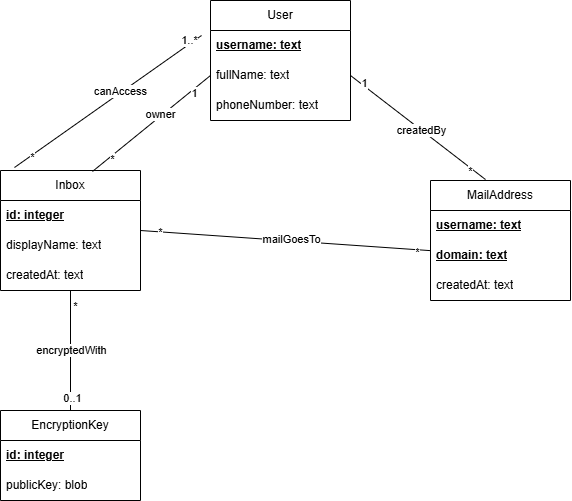
\includegraphics[width=1\textwidth]{model/original_uml_class_diagram.png}
    \caption{The original UML class diagram for the email system.}
    \label{fig:originalUMLClassDiagram}
\end{figure}

\begin{figure}[htb]
    \centering
    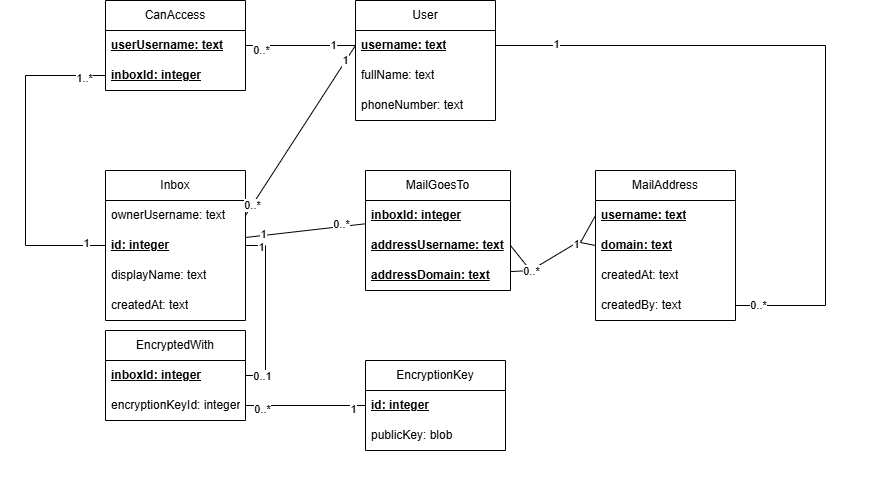
\includegraphics[width=1\textwidth]{model/database_friendly.png}
    \caption{The database model for the email system.}
    \label{fig:originalDatabaseModel}
\end{figure}

To further exemplify the database model we will also provide an instance of the database model in figure \ref{fig:instanceDatabaseModel}. This instance will be used in the examples below to show how to insert data using the SQLite Implementation Tools.

\begin{figure}[htb]
    \centering
    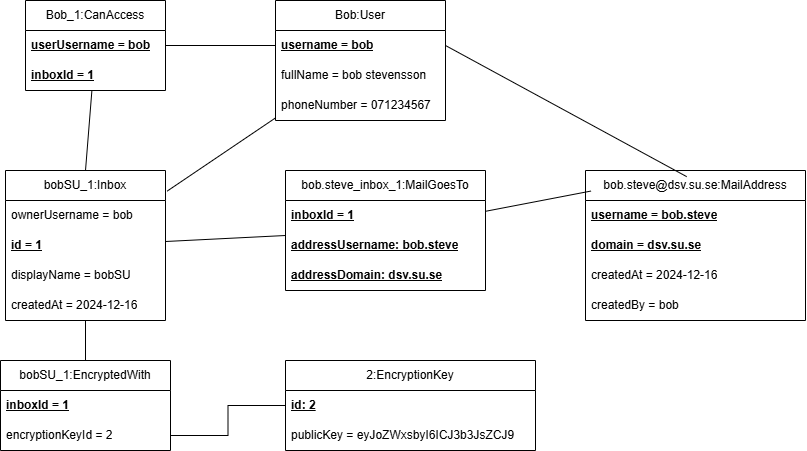
\includegraphics[width=1\textwidth]{model/instance.png}
    \caption{An instance of the database model for the email system.}
    \label{fig:instanceDatabaseModel}
\end{figure}

\section{The SQLite Implementation Tools}
\label{sqliteImplementationTools}
The following tools will be presented in this document:
\begin{itemize}
    \item DBeaver Community (see \autoref{dbeaverCommunity})
    \item SQLiteStudio (see \autoref{sqliteStudio})
    \item SQLite ERD (see \autoref{sqliteERD})
\end{itemize}

\section{DBeaver Community}
\label{dbeaverCommunity}

\subsection{Relevant Known Issues}
\label{dbeaverKnownIssues}

\subsubsection{Bad Primary Key due to auto increment}
When creating an integer column in DBeaver Community with the ``auto increment'' box checked the SQL generated will have a PK constraint created twice. This will result in an error when trying to persist the changes since a table can only have one PRIMARY KEY constraint. The following code is generated by DBeaver Community when trying to persist the changes:
\begin{lstlisting}[caption={Bad Primary Key due to auto increment in DBeaver}]
CREATE TABLE BadPK (
	Column1 INTEGER NOT NULL PRIMARY KEY AUTOINCREMENT,
	CONSTRAINT BadPK_PK PRIMARY KEY (Column1)
);
\end{lstlisting}
The solution to this is to never use the ``auto increment box'' (for a SQLite database in DBeaver) when creating a PK in the program. Unchecking the box will instead yield the following code:
\begin{lstlisting}[caption={Ok Primary Key in DBeaver if auto increment is unchecked}]
CREATE TABLE GoodPK (
	Column1 INTEGER NOT NULL,
	CONSTRAINT GoodPK_PK PRIMARY KEY (Column1)
);
\end{lstlisting}
For more information on why this is the case see \cite{dbeaver_issue_18491}.

\subsection{Common Problems}
\label{dbeaverCommonProblems}
% TODO: Usertests!

\subsection{Implementation of the Database Model}
\label{dbeaverImplementation}

\subsubsection{Creating a Database}
\label{dbeaverCreatingDatabase}

\subsubsection{Creating a Table}
\label{dbeaverCreatingTable}

\subsubsection{Foreign Keys}
\label{dbeaverForeignKeys}

\subsubsection{Inserting Data}
\label{dbeaverInsertingData}

\subsubsection{Querying Data}
\label{dbeaverQueryingData}


\section{SQLiteStudio}
\label{sqliteStudio}

\subsection{Relevant Known Issues}
\label{sqliteStudioKnownIssues}

\subsection{Common Problems}
\label{sqliteStudioCommonProblems}
% TODO: Usertests!

\subsection{Implementation of the Database Model}
\label{sqliteStudioImplementation}

\subsubsection{Creating a Database}
\label{sqliteStudioCreatingDatabase}

\subsubsection{Creating a Table}
\label{sqliteStudioCreatingTable}

\subsubsection{Foreign Keys}
\label{sqliteStudioForeignKeys}

\subsubsection{Inserting Data}
\label{sqliteStudioInsertingData}

\subsubsection{Querying Data}
\label{sqliteStudioQueryingData}
% queries should be saved as Views

\section{SQLite ERD}
\label{sqliteERD}
SQLite ERD is an application that can be used to create Entity Relationship Diagrams (ERDs) for SQLite databases. The application is platform independent and is used within a web browser. The application can be found at \url{https://sqlite-erd.e-su.se/}. For the interested reader the source code can be found at \url{https://github.com/Edwinexd/sqlite-erd}.

The application supports most common file formats for SQLite databases and the only requirement is that the file is a SQLite database of version 3.

% TODO: include figure generated from sqlite-erd

\section{Final Words}
\label{finalWords}
If you have any questions or issues with the tools presented in this document or the document itself please create an issue at \url{https://github.com/Edwinexd/db-sqlite-tools/issues}.


\pagebreak
\bibliographystyle{plain}
\bibliography{bibtex}
\bibdata{bibtex}

\end{document}
